%!TEX root = main.tex

\section{Exercises}

\begin{problem}[Basic]
Find an example of a function $f\colon \field{R} \to \field{R}$ (different from the function in Example \ref{example:NewtonRaphsonloop}) with a unique root at $x=0$ for which the Newton-Raphson sequence is a loop no matter the initial guess $x_0\neq 0$: $x_{2n}=x_0$, $x_{2n+1}=-x_0$ for all $n \in \field{N}$.
\end{problem}

\begin{problem}[Intermediate]
Consider the function 
\begin{equation*}
f(x) = 9x -4\log(x-7).
\end{equation*}
We wish to study the behavior of Newton-Raphson to find approximations to the critical points of this function.
\begin{enumerate}
	\item Find the domain $D$ of $f$.
	\item Find the global minimum of $f$ analytically.
	\item Compute an exact formula for the Newton-Raphson iterate $x_{n+1}$ for an initial guess $x_0 \in D$.
	\item Compute five iterations of the Newton-Raphson method starting at each of the following initial guesses:
	\begin{enumerate}
		\item $x_0 = 7.4$.
		\item $x_0 = 7.2$.
		\item $x_0 = 7.01$.
		\item $x_0 = 7.8$.
		\item $x_0 = 7.88$.
	\end{enumerate}
	\item Prove that the Newton-Raphson method converges to the optimal solution for any initial guess $x_0 \in (7,7.8888)$.
	\item What is the behavior of the Newton-Raphson method if the initial guess is not in the interval $(7,7.8888)$?
\end{enumerate}
\end{problem}

\begin{problem}[Intermediate]
Consider the function 
\begin{equation*}
f(x) = 6x -4\log(x-2) -3\log(25-x).
\end{equation*}
We wish to study the behavior of Newton-Raphson to find approximations to the critical points of this function.
\begin{enumerate}
	\item Find the domain $D$ of $f$.
	\item Find the global minimum of $f$ analytically. 
	\item Compute an exact formula for the Newton-Raphson iterate $x_{n+1}$ for an initial guess $x_0 \in D$.
	\item Compute five iterations of the Newton-Raphson method starting at each of the following initial guesses:
	\begin{enumerate}
		\item $x_0 = 2.6$.
		\item $x_0 = 2.7$.
		\item $x_0 = 2.4$.
		\item $x_0 = 2.8$.
		\item $x_0 = 3$.
	\end{enumerate}
	\item Prove that the Newton-Raphson method converges to the optimal solution for any initial guess $x_0 \in (2,3.05)$.
	\item What is the behavior of the Newton-Raphson method if the initial guess is not in the interval $(2,3.05)$?
\end{enumerate}
\end{problem}

\begin{problem}[CAS]
Design a process in \texttt{desmos.com} to test the search for critical points given by the recursion formulas produced by Newton's method.
\begin{figure}[ht!]
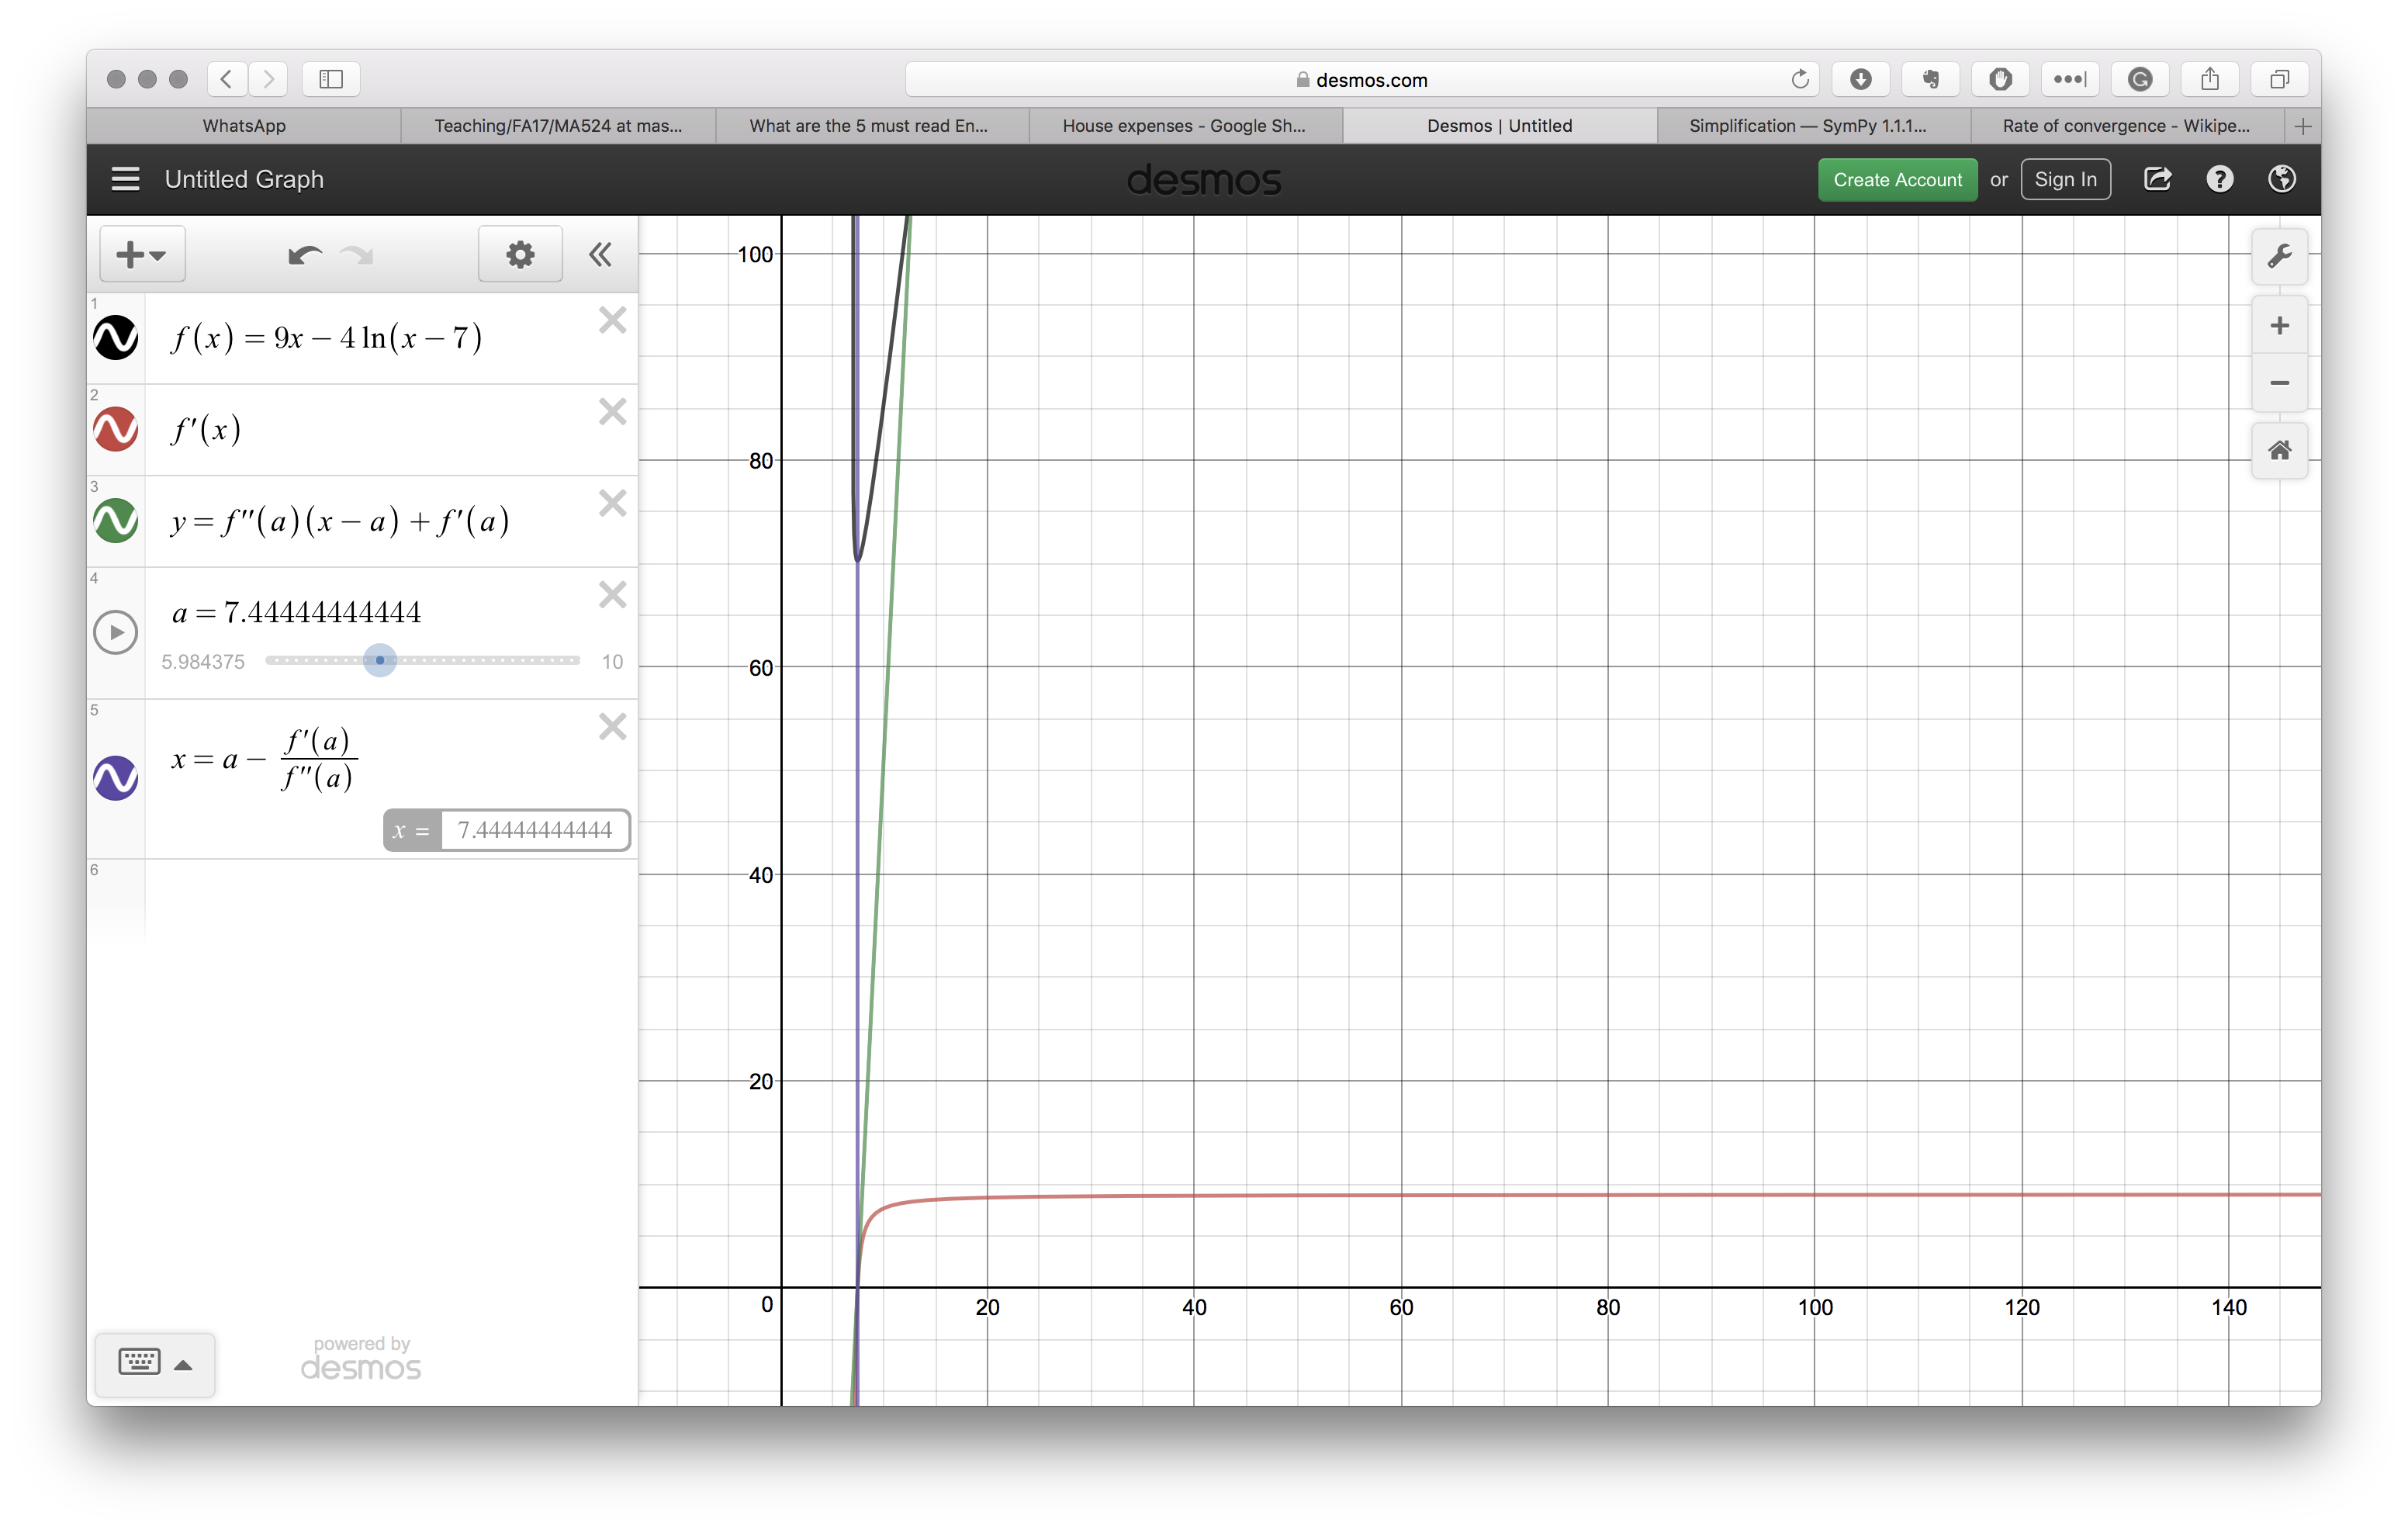
\includegraphics[width=\linewidth]{desmos.png}
\caption{Newton method in \texttt{desmos.com}}
\label{figure:desmosNewton}
\end{figure}
\end{problem}

\begin{problem}[Advanced]
Prove Theorems \ref{theorem:SteepestDescentDescends}, and \ref{theorem:SteepestDescentConvergesToCritical}.
\end{problem}
